\documentclass[border=6pt]{standalone}
\usepackage{tikz}
\begin{document}
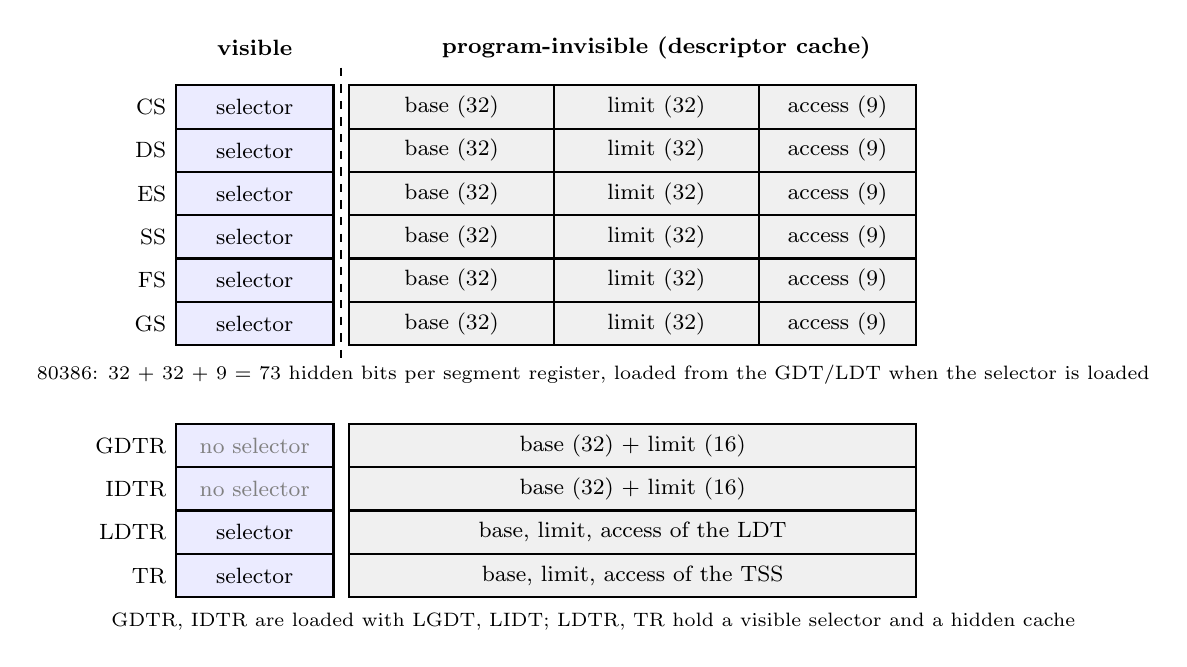
\begin{tikzpicture}[font=\small,
 c/.style={draw,thick,minimum height=0.55cm,font=\footnotesize,inner sep=1pt}]
\node[font=\footnotesize\bfseries] at (1.0,0.75) {visible};
\node[font=\footnotesize\bfseries] at (6.1,0.75) {program-invisible (descriptor cache)};
\foreach \r/\y in {CS/0,DS/-0.55,ES/-1.1,SS/-1.65,FS/-2.2,GS/-2.75} {
  \node[anchor=east,font=\footnotesize] at (0.0,\y) {\r};
  \node[c,fill=blue!8,minimum width=2.0cm] at (1.0,\y) {selector};
  \node[c,fill=gray!12,minimum width=2.6cm] at (3.5,\y) {base (32)};
  \node[c,fill=gray!12,minimum width=2.6cm] at (6.1,\y) {limit (32)};
  \node[c,fill=gray!12,minimum width=2.0cm] at (8.4,\y) {access (9)};
}
\draw[thick,dashed] (2.1,0.5) -- (2.1,-3.2);
\node[font=\scriptsize,anchor=north] at (5.3,-3.15) {80386: 32 + 32 + 9 = 73 hidden bits per segment register, loaded from the GDT/LDT when the selector is loaded};
\begin{scope}[yshift=-4.3cm]
\foreach \r/\y/\v/\h in {GDTR/0/{\textcolor{gray}{no selector}}/{base (32) + limit (16)},IDTR/-0.55/{\textcolor{gray}{no selector}}/{base (32) + limit (16)},LDTR/-1.1/selector/{base, limit, access of the LDT},TR/-1.65/selector/{base, limit, access of the TSS}} {
  \node[anchor=east,font=\footnotesize] at (0.0,\y) {\r};
  \node[c,fill=blue!8,minimum width=2.0cm] at (1.0,\y) {\v};
  \node[c,fill=gray!12,minimum width=7.2cm] at (5.8,\y) {\h};
}
\node[font=\scriptsize,anchor=north] at (5.3,-2.0) {GDTR, IDTR are loaded with LGDT, LIDT; LDTR, TR hold a visible selector and a hidden cache};
\end{scope}
\end{tikzpicture}
\end{document}
